\chapter{Materials and Methods}

This chapter focus on describing the used materials and methods utilized in this thesis. The acoustic emission tests (Section \ref{sec:AETest}) had 3 separate data acquisition systems, one using an industrial device (DISP-16C) made by Physical Acoustics (PAC), one with another industrial device (AMSY-5) made by Vallen Systems and a custom one denominated Streaming.

Both Streaming and Vallen data were analysed throughout the project duration, however, this thesis concentrates solely on the Streaming data. Both are similar in the way that they acquire temporal data from the AE (not its parameters), however, the AE waveforms captured by the Vallen system had several disadvantages when compared to the Streaming counterpart.

The Vallen data is a collection of fixed length AEs concatenated to form a $L \times N$ matrix where $L$ is the AE length and $N$ the number of captured AEs. This matrix was provided as a MATLAB formatted data file (.MAT) containing the waveform using 64-bit double-precision floating-point format. Unfortunately, this system is not guaranteed to capture all waveforms, this severely hinders some essential preprocessing stages (Sections \ref{sec:TOFDRemoval} and \ref{sec:bombRemoval}), making it a rather unreliable (the captured AE may not be from the crack propagation) and with no means of improving its reliability, therefore all of the Vallen data was discarded.

Thus, this chapter begins detailing the destructive test done, extends to the raw data format used, describes all the preprocessing done and the reasoning behind it, then details the waveform capture procedure all the way to creating the final dataset used to train a neural network model (Section \ref{sec:ann}) with parameters from both the AE temporal data and its frequency spectrum.


\section{Acoustic Emission Test} \label{sec:AETest}

The test uses a close-ended steel (API XL 60 series) cylinder with $20$ inch diameter, $40$ metre length and $1.45$ centimetres of thickness, a semi-elliptical pre-crack extending until half of its thickness (approximately $0.7 cm$) was inserted at half its length.

%mention the rubber cape !!!!!!!!!!

The hydrostatic test consists of a gradual increase of pressure (after filling the tube) followed by plateaus until it bursts (Figure \ref{fig:pressure_time}). In total, $4$ (four) tests were done, with the first one discarded since it did not burst. They were denominated CP1, CP2, CP3 and CP4 respectively.

\begin{figure}[H]
	\centering
	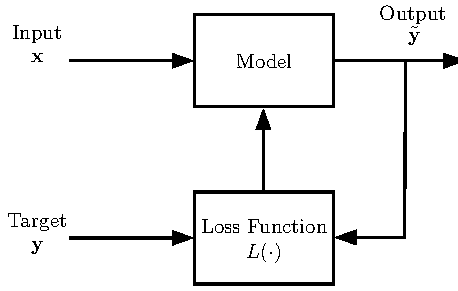
\includegraphics[width=0.1\textwidth]{sup_learning_schematic}
	\caption{Pressure and Crack Dimension for Test CPX}
	\label{fig:pressure_time}
\end{figure}

A sensor array was then disposed on top of the naked steel and the rubber cape (Figure \ref{fig:sensor_disposition}) throughout the tube's length surrounding the crack.
%mention TOFD -> AE sensor or AE sensor -> TOFD ?

\begin{figure}[H]
	\centering
	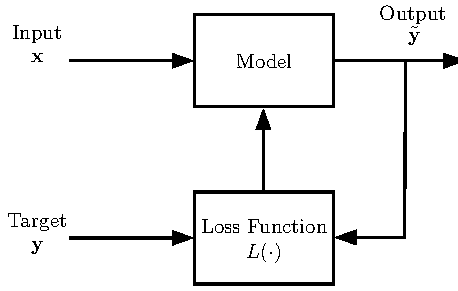
\includegraphics[width=0.1\textwidth]{sup_learning_schematic}
	\caption{Sensor Array Disposition for Test CP3}
	\label{fig:sensor_disposition}
\end{figure}

\section{Streaming Raw Data}

\section{Preprocessing}
\subsection{Resolution Analysis}

\subsection{TOFD Removal} \label{sec:TOFDRemoval}
\subsection{Pressure Bomb Removal} \label{sec:bombRemoval}

\section{Wave Capture}
\subsection{Acoustic Emission Parameters}
\subsection{Frequency Data}

\section{Database Structure}

\section{Model Definition}

\subsection{Network Size}
\subsection{\textit{Transition Time Estimation}}
\subsection{Relevance Analysis}

